\chapter{Die technische Implementierung von Webservices}
\label{cha:TechnischeImplementierungWebservices}
In den folgenden drei Kapiteln wird der Autor eine einfache Webservice-Umgebung aufbauen, um zu zeigen, wie Webservices in der Praxis angeboten, konsumiert und orchestriert werden können. Hierzu verwendet er ausschließlich Open-Source-Software, im Speziellen \NeuerBegriff{Apache Tomcat}\footnote{Website: \url{http://tomcat.apache.org/}} als Servlet-Engine, \NeuerBegriff{Apache Axis2}\footnote{Website: \url{http://ws.apache.org/axis2/}} als SOAP-Engine und \NeuerBegriff{ActiveBPEL}\footnote{Website: \url{http://www.activebpel.org/}} als Workflow-System. Die Installation und Konfiguration der benötigten Anwendungen wird in Kapitel \ref{sec:Werkzeuge} im Anhang beschrieben. Die komplette Umgebung inkl. der vom Autor erstellten Webservices befindet sich als virtuelle Maschine auf der dieser Arbeit beigelegten DVD. Im Folgenden wird der DNS-Name \Code{linux-ws} als Bezeichnung für den Webservice-Server verwendet.

\section{Anbieten eines Webservice}
\label{sec:AnbietenEinesWebservices}
Mit Hilfe von Apache Axis2 können Webservices sehr einfach auf Basis von normalen Java-Klassen angeboten werden. Es ist lediglich eine zusätzliche XML-Datei namens \Datei{META-INF/services.xml} nötig, in der die zu veröffentlichenden Klassen und Methoden beschrieben werden. Abbildung \ref{fig:HelloWorldStruktur} zeigt die Struktur eines einfachen \Webservice{HelloWorld}-Webservice.

\begin{figure}[htb]
\centering
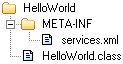
\includegraphics[width=0.3\textwidth]{HelloWorldStruktur.jpg}
\caption{\Webservice{HelloWorld}-Webservice: Dateistruktur}
\label{fig:HelloWorldStruktur}
\end{figure}

Die Klasse \Code{HelloWorld} besitzt nur die Methode \Code{SayHello}, die den \Datentyp{String} \Code{Hello World!} zurückgibt. Sie wird in Listing \ref{lst:HelloWorldJava} gezeigt. 

\lstset{language=Java, basicstyle=\footnotesize, showstringspaces=false, tabsize=2}
\lstinputlisting[label=lst:HelloWorldJava,caption=\Webservice{HelloWorld}-Webservice: Java-Klasse \Code{HelloWorld}]{DVD/Listings/HelloWorld/HelloWorld.java}
